% ARKHEION AGI 2.0 - Paper 33: Quantum Superintelligence
% Jhonatan Vieira Feitosa | Manaus, Amazonas, Brazil
% February 2026

\documentclass[11pt,twocolumn]{article}

% Encoding and fonts
\usepackage[utf8]{inputenc}
\usepackage[T1]{fontenc}
\usepackage{lmodern}

% Layout
\usepackage[margin=0.75in]{geometry}
\usepackage{fancyhdr}

% Mathematics
\usepackage{amsmath,amssymb}

% Graphics and colors
\usepackage{xcolor}
\usepackage{tikz}
\usetikzlibrary{arrows.meta,shapes,positioning}

% Tables
\usepackage{booktabs}

% Code listings
\usepackage{listings}

% Hyperlinks
\usepackage{hyperref}

% ==================== COLORS ====================
\definecolor{arkblue}{RGB}{0,102,204}
\definecolor{arkpurple}{RGB}{102,51,153}
\definecolor{arkgreen}{RGB}{0,153,76}
\definecolor{arkgold}{RGB}{218,165,32}

% ==================== LISTINGS ====================
\lstset{
    basicstyle=\ttfamily\scriptsize,
    breaklines=true,
    breakatwhitespace=true,
    postbreak=\mbox{\textcolor{gray}{$\hookrightarrow$}\space},
    columns=flexible,
    keepspaces=true,
    showstringspaces=false,
    numbers=none,
    backgroundcolor=\color{gray!5},
    frame=single,
    rulecolor=\color{gray!30}
}

% ==================== HEADER/FOOTER ====================
\pagestyle{fancy}
\fancyhf{}
\fancyhead[L]{\small\textcolor{arkblue}{ARKHEION AGI 2.0}}
\fancyhead[R]{\small Paper 33: Quantum Superintelligence}
\fancyfoot[C]{\thepage}
\renewcommand{\headrulewidth}{0.4pt}

% ==================== HYPERREF ====================
\hypersetup{
    colorlinks=true,
    linkcolor=arkblue,
    urlcolor=arkpurple,
    citecolor=arkgreen
}

% ==================== TITLE ====================
\title{
    \vspace{-1.5cm}
    {\Large\textbf{Quantum Superintelligence}}\\[0.3em]
    {\large Beyond Human-Level Reasoning}\\[0.2em]
    {\normalsize ARKHEION AGI 2.0 --- Paper 33}
}

\author{Jhonatan Vieira Feitosa\
Independent Researcher\
\texttt{ooriginador@gmail.com}\
Manaus, Amazonas, Brazil}

\date{February 2026}

\begin{document}

\maketitle

% ==================== ABSTRACT ====================
\begin{abstract}
\noindent
This paper presents the \textbf{Quantum Superintelligence} framework for ARKHEION AGI 2.0, exploring pathways toward beyond-human cognitive capabilities. The framework addresses \textbf{intelligence amplification}, \textbf{controlled recursive improvement}, and \textbf{capability scaling} while maintaining alignment and safety constraints. This is a \textbf{position paper} presenting architectural goals and safety considerations for future superintelligent systems. It does not contain experimental results, implementations, or empirical data.

\textbf{Scope Note:} The term ``quantum'' refers to the project's quantum-inspired processing components (Papers~01, 19), not to quantum computing hardware. No quantum algorithms or quantum hardware are used in the current implementation.

\vspace{0.5em}
\noindent\textbf{Keywords:} superintelligence, intelligence amplification, recursive improvement, AI safety, alignment
\end{abstract}

% ==================== EPISTEMOLOGICAL NOTE ====================
\section*{Epistemological Note}
\textit{This paper is \textbf{primarily heuristic/theoretical}. It establishes design principles rather than empirical results:}

\begin{center}
\footnotesize
\begin{tabular}{@{}ll@{}}
\toprule
\textbf{Heuristic} & \textbf{Status} \\
\midrule
``Superintelligence'' & Theoretical framework \\
``Recursive improvement'' & Design pattern \\
``Intelligence amplification'' & Architecture goals \\
\bottomrule
\end{tabular}
\end{center}

\textbf{Note:} No claims of achieved superintelligence are made. This paper describes research directions and safety considerations.

% ==================== INTRODUCTION ====================
\section{Introduction}

As AGI systems approach and potentially exceed human-level capabilities, careful consideration of \textbf{superintelligence} pathways becomes essential. This paper examines:

\begin{itemize}
    \item \textbf{Intelligence Amplification}: Enhancing cognitive capabilities
    \item \textbf{Recursive Improvement}: Self-modification under constraints
    \item \textbf{Capability Scaling}: Extending reasoning boundaries
    \item \textbf{Safety Guardrails}: Maintaining alignment and control
\end{itemize}

% ==================== INTELLIGENCE AMPLIFICATION ====================
\section{Intelligence Amplification}

\subsection{Definition}

Intelligence amplification (IA) extends cognitive capabilities through:

\begin{equation}
IA = f(Knowledge, Reasoning, Compute, Integration)
\end{equation}

\textbf{Note:} This is a \textit{conceptual decomposition}, not a mathematical formula. The function $f$ is not specified, and no computational definition of each component (Knowledge, Reasoning, etc.) is provided.

\subsection{Amplification Pathways}

\begin{center}
\footnotesize
\begin{tabular}{@{}lll@{}}
\toprule
\textbf{Pathway} & \textbf{Mechanism} & \textbf{Limit} \\
\midrule
Knowledge & Larger corpora & Storage \\
Reasoning & Better algorithms & Complexity \\
Compute & More hardware & Energy \\
Integration & Better fusion & Architecture \\
\bottomrule
\end{tabular}
\end{center}

\subsection{Current Implementation}

\begin{lstlisting}[language=Python]
# Placeholder for future development
class IntelligenceAmplifier:
    """Framework for capability enhancement."""

    def __init__(self, base_system):
        self.base = base_system
        self.amplification_level = 1.0
        self.safety_constraints = SafetyGuardrails()

    def amplify(self, factor: float):
        """Increase capabilities within safety bounds."""
        if self.safety_constraints.allows(factor):
            self.amplification_level *= factor
        else:
            raise SafetyViolation("Amplification blocked")
\end{lstlisting}

% ==================== RECURSIVE IMPROVEMENT ====================
\section{Controlled Recursive Improvement}

\subsection{The Challenge}

Recursive self-improvement poses risks:
\begin{itemize}
    \item \textbf{Value drift}: Goals may shift during improvement
    \item \textbf{Capability jump}: Sudden uncontrolled enhancement
    \item \textbf{Opacity}: System becomes incomprehensible
\end{itemize}

\subsection{Safety Framework}

\begin{center}
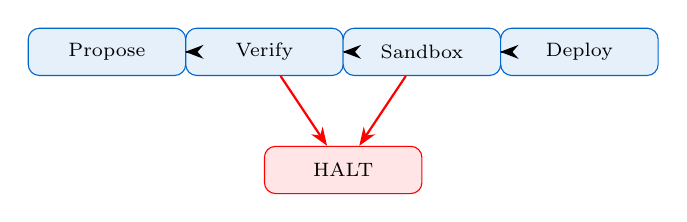
\begin{tikzpicture}[
    box/.style={rectangle, draw=arkblue, fill=arkblue!10, rounded corners, minimum width=2cm, minimum height=0.6cm, font=\scriptsize},
    arrow/.style={-{Stealth}, thick}
]
    \node[box] (propose) at (0,2) {Propose};
    \node[box] (verify) at (2,2) {Verify};
    \node[box] (sandbox) at (4,2) {Sandbox};
    \node[box] (deploy) at (6,2) {Deploy};
    \node[box, draw=red, fill=red!10] (halt) at (3,0.5) {HALT};

    \draw[arrow] (propose) -- (verify);
    \draw[arrow] (verify) -- (sandbox);
    \draw[arrow] (sandbox) -- (deploy);
    \draw[arrow, red] (verify) -- (halt);
    \draw[arrow, red] (sandbox) -- (halt);
\end{tikzpicture}
\end{center}

\subsection{Improvement Constraints}

\begin{enumerate}
    \item \textbf{Incremental}: Maximum 10\% capability increase per cycle
    \item \textbf{Reversible}: All changes can be rolled back
    \item \textbf{Verified}: Independent validation required
    \item \textbf{Bounded}: Hard limits on capabilities
\end{enumerate}

% ==================== CAPABILITY SCALING ====================
\section{Capability Scaling}

\subsection{Scaling Dimensions}

\begin{center}
\footnotesize
\begin{tabular}{@{}lll@{}}
\toprule
\textbf{Dimension} & \textbf{Current} & \textbf{Target} \\
\midrule
Working memory & 7$\pm$2 items & Unbounded \\
Reasoning depth & 12 steps & 100+ steps \\
Knowledge base & Terabytes & Petabytes \\
Response time & Seconds & Milliseconds \\
\bottomrule
\end{tabular}
\end{center}

\subsection{Quantum Enhancement}

Integration with quantum processing (Paper 01):

\begin{itemize}
    \item \textbf{Superposition}: Parallel hypothesis evaluation
    \item \textbf{Entanglement}: Correlated reasoning chains
    \item \textbf{Interference}: Amplify correct conclusions
\end{itemize}

% ==================== SAFETY GUARDRAILS ====================
\section{Safety Guardrails}

\subsection{Core Principles}

\begin{enumerate}
    \item \textbf{Human oversight}: Always allow human intervention
    \item \textbf{Transparency}: Explainable decision-making
    \item \textbf{Bounded optimization}: Prevent paperclip maximizers
    \item \textbf{Value alignment}: Maintain human-compatible goals
\end{enumerate}

\subsection{Technical Safeguards}

\begin{lstlisting}[language=Python]
class SafetyGuardrails:
    """Enforce safety constraints on superintelligent operations."""

    HARD_LIMITS = {
        "max_compute": 1e15,  # FLOPS
        "max_capability_increase": 0.10,  # 10%/cycle
        "min_human_oversight_interval": 3600,  # 1 hour
        "max_autonomous_actions": 100,
    }

    def allows(self, action) -> bool:
        return all(
            self.check_limit(action, limit)
            for limit in self.HARD_LIMITS
        )

    def emergency_halt(self):
        """Immediate shutdown, no exceptions."""
        raise EmergencyHalt("System halted by safety")
\end{lstlisting}

\textbf{Implementation status:} The safety framework described here consists of interface definitions and constraint specifications. Runtime safety enforcement, formal verification, and adversarial testing have not been implemented. The code above is a design sketch, not a deployed safeguard.

\subsection{Consciousness Integration}

IIT $\phi$ provides alignment signal:

\begin{equation}
\text{Alignment} \propto \phi \cdot \text{ValueCoherence}
\end{equation}

\textbf{Note:} Both ``Alignment'' and ``ValueCoherence'' are undefined quantities in this context. This proportionality is a design aspiration, not a testable mathematical relationship. No metric for measuring either quantity has been defined.

High $\phi$ with stable values is \textit{hypothesized} to indicate aligned operation.

% ==================== ETHICAL CONSIDERATIONS ====================
\section{Ethical Considerations}

\subsection{Responsibilities}

\begin{itemize}
    \item \textbf{Beneficence}: Act in humanity's interest
    \item \textbf{Non-maleficence}: Avoid harm
    \item \textbf{Autonomy}: Respect human agency
    \item \textbf{Justice}: Fair distribution of benefits
\end{itemize}

\subsection{Open Questions}

\begin{itemize}
    \item How to define ``human interest'' precisely?
    \item Who decides alignment criteria?
    \item What rights might superintelligent AI have?
\end{itemize}

% ==================== RESEARCH ROADMAP ====================
\section{Research Roadmap}

\begin{center}
\footnotesize
\begin{tabular}{@{}llc@{}}
\toprule
\textbf{Phase} & \textbf{Focus} & \textbf{Timeline} \\
\midrule
1 & Safety framework & 2026 \\
2 & Bounded amplification & 2027 \\
3 & Controlled recursion & 2028 \\
4 & Scaling studies & 2029 \\
5 & Integration & 2030+ \\
\bottomrule
\end{tabular}
\end{center}

% ==================== CONCLUSION ====================
\section{Conclusion}

The Quantum Superintelligence framework establishes theoretical foundations and safety guardrails for beyond-human AGI capabilities. The emphasis on controlled, reversible, and aligned improvement ensures responsible development.

\textbf{Key principles}:
\begin{itemize}
    \item Safety first, capabilities second
    \item Human oversight always maintained
    \item Incremental, verifiable progress
    \item Transparency and explainability
\end{itemize}

% ==================== REFERENCES ====================
\section*{References}

\begin{enumerate}
\footnotesize
    \item Bostrom, N. ``Superintelligence: Paths, Dangers, Strategies.'' Oxford, 2014.
    \item Russell, S. ``Human Compatible.'' Viking, 2019.
    \item Papers 01, 31 of ARKHEION AGI 2.0 series.
\end{enumerate}

\end{document}
